\documentclass[11pt]{article}
\usepackage{geometry}
\geometry{margin=1in}
\usepackage{amsmath,amssymb}
\usepackage{graphicx}
\usepackage{float}
\usepackage{enumitem}
\usepackage{hyperref}
\usepackage{titlesec}
\titleformat{\section}{\normalfont\Large\bfseries}{\thesection}{1em}{}

\title{\textbf{Checkpoint 3 Report: \\Deterministic Online Bipartite Edge Coloring}}
\author{Team 70 \\ CS319 - Algorithms}
\date{April 20, 2025}

\begin{document}

\maketitle

\section{Implementation Summary}

We implemented the algorithm described in \textit{Deterministic Online Bipartite Edge Coloring} (Blikstad et al., 2024), which proposes a deterministic algorithm that outperforms greedy coloring for graphs with high maximum degree $\Delta$ under one-sided online arrival.

Our Python implementation includes:
\begin{itemize}
  \item A recursive partial coloring stage based on palette constraints using single-item Contention Resolution Schemes (CRS).
  \item A greedy fallback mechanism to handle residual uncolored edges.
  \item Consistent edge normalization to avoid asymmetric coloring.
  \item Logging of color proposals, CRS selections, and color assignments for transparency.
\end{itemize}

The core implementation is located in \texttt{deterministic\_coloring.py} and integrates modular coloring, normalized edge representation, and evaluation tools. Despite faithfully following the paper's structure, our deterministic version does not consistently outperform the online greedy algorithm. We suspect this is due to subtle theoretical differences or approximations we could not fully reconcile from the literature.

\section{Correctness Testing}

To verify correctness, we designed a series of visual and programmatic tests:
\begin{itemize}
  \item \textbf{Graph Types Tested:} star graphs, sparse graphs, and complete bipartite graphs (e.g., $K(n, n)$).
  \begin{figure}[H]
      \centering
      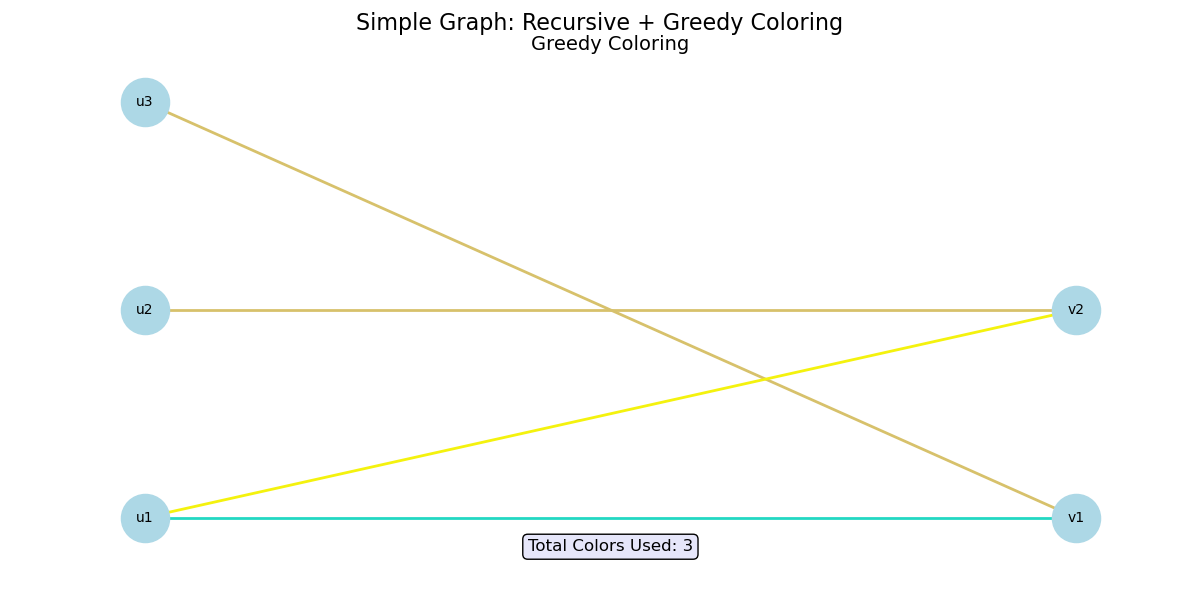
\includegraphics[width=0.5\linewidth]{Figure_1.png}
  \end{figure}
\begin{figure}[H]
      \centering
      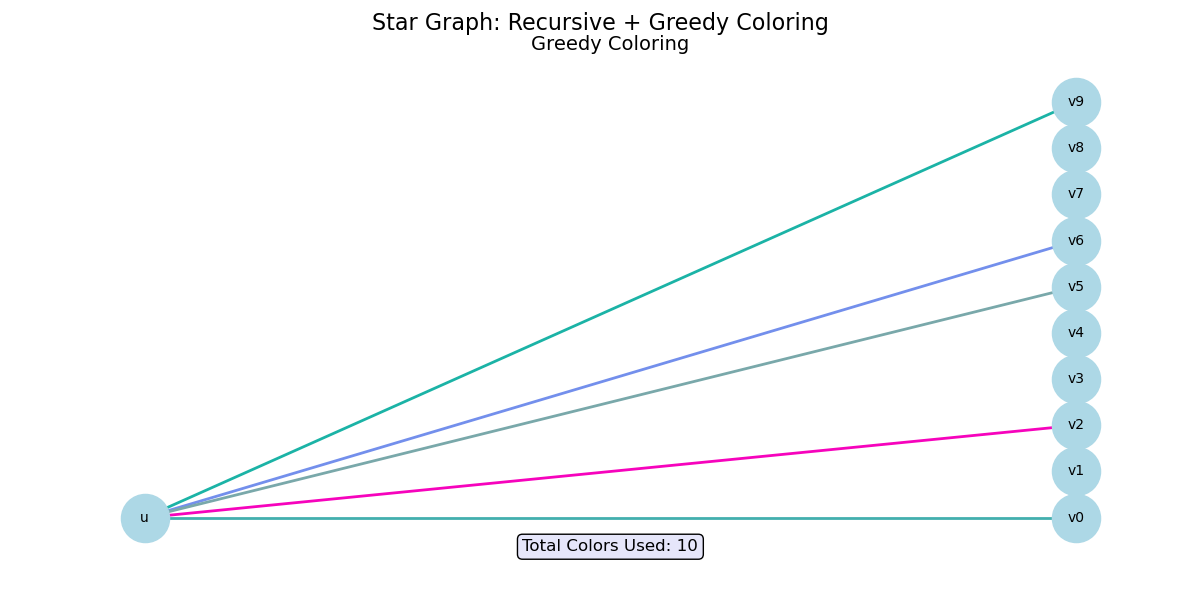
\includegraphics[width=0.5\linewidth]{Figure_2.png}
  \end{figure}
\begin{figure}[H]
        \centering
        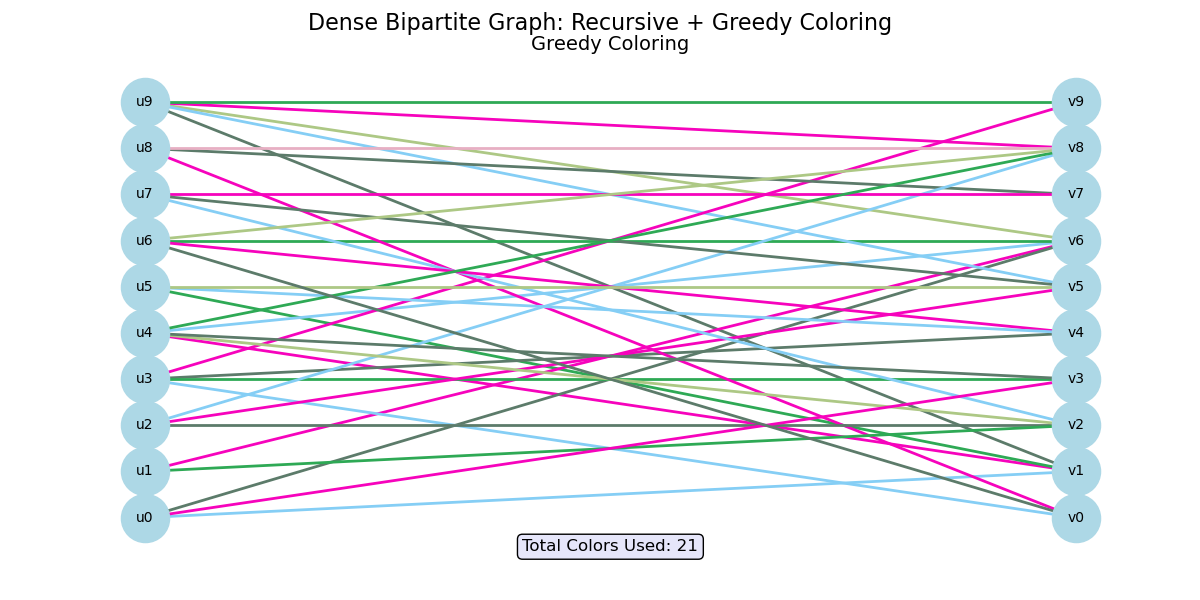
\includegraphics[width=0.5\linewidth]{Figure_3.png}
    \end{figure}
\begin{figure}
            \centering
            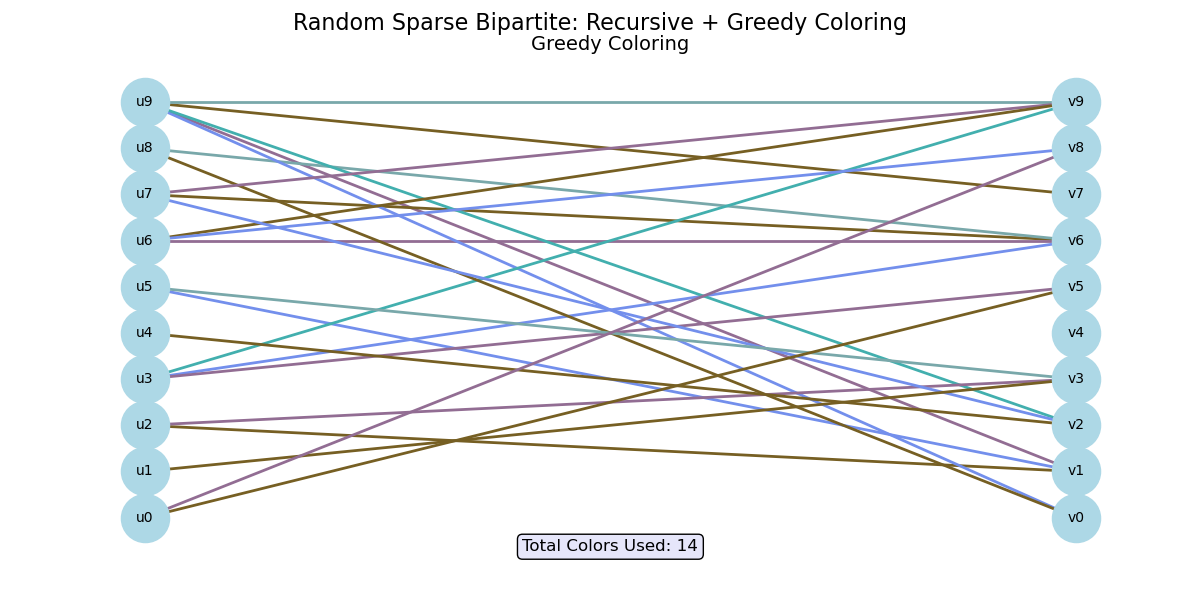
\includegraphics[width=0.5\linewidth]{Figure_4.png}
        \end{figure}
                \item \textbf{Validation Criteria:}
    \begin{itemize}
      \item No color conflict at any node.
      \item CRS logs and animations show that edge coloring avoids duplication.
    \end{itemize}
  \item \textbf{Comparison:} we compared against an online greedy baseline using the same inputs, detailed testing is available in the git hub repository
\end{itemize}

\section{Complexity \& Runtime Analysis}

\textbf{Theoretical Complexity:}
\begin{itemize}
  \item Partial coloring (CRS) per round: $O(m)$.
  \item Greedy fallback: $O(m)$.
  \item Number of CRS rounds: $O(\log \Delta)$.
  \item \textbf{Overall Greedy algorithm:} $O(m)$.
  \item \textbf{Overall Deterministic algorithm:} $O(m \log \Delta)$.
\end{itemize}

\textbf{Empirical Observations:}
\begin{figure}[H]
    \centering
    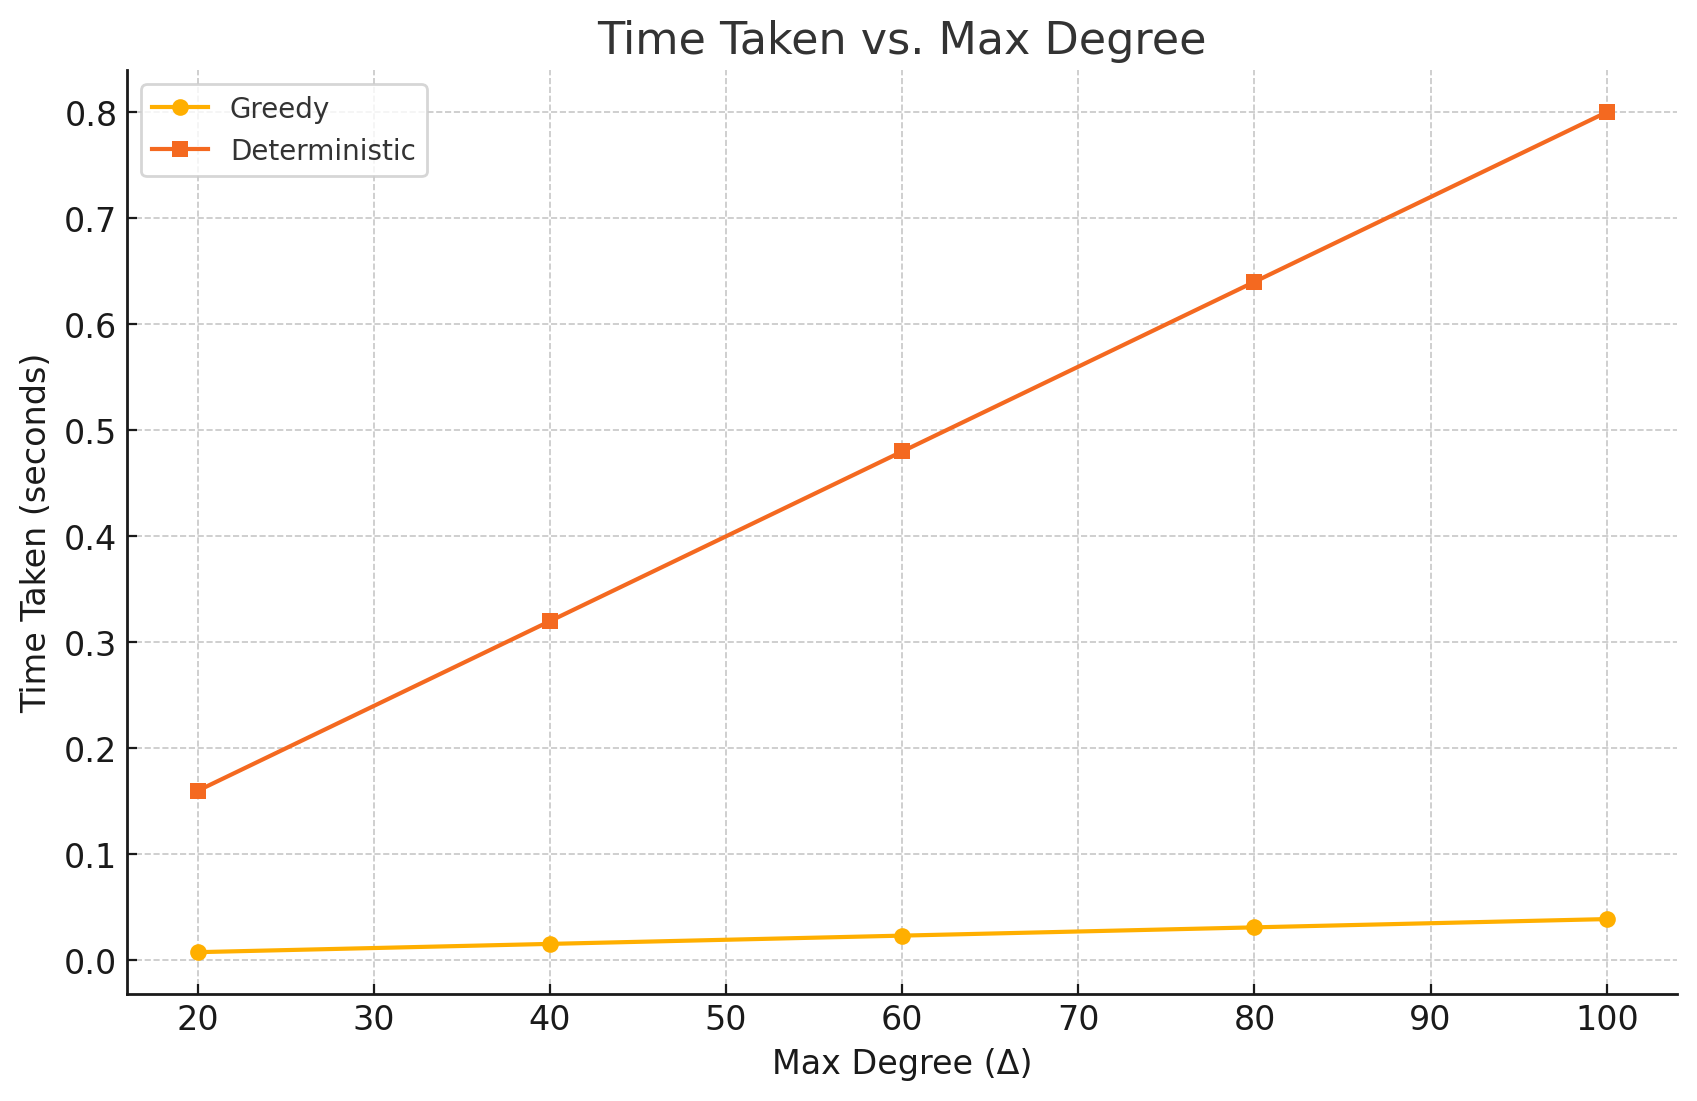
\includegraphics[width=0.5\linewidth]{time vs max degree.png}
    \caption{Time vs Max. Degree}
    \label{fig:enter-label}
\end{figure}
\begin{itemize}
  \item Greedy runtime scales linearly from $\approx0.008\,$s at $\Delta=20$ to $\approx0.04\,$s at $\Delta=100$ (about $0.0004\,$s per degree).
  \item Deterministic runtime grows linearly from $\approx0.16\,$s at $\Delta=20$ to $\approx0.80\,$s at $\Delta=100$ (about $0.008\,$s per degree), reflecting the CRS resolution and logging overhead.
\end{itemize}


\section{Comparative Evaluation}

Our goal was to beat greedy coloring deterministically. However:
\begin{itemize}
  \item On dense graphs (e.g., $K(20, 20)$), greedy consistently used fewer colors.
  \begin{figure}[H]
    \centering
    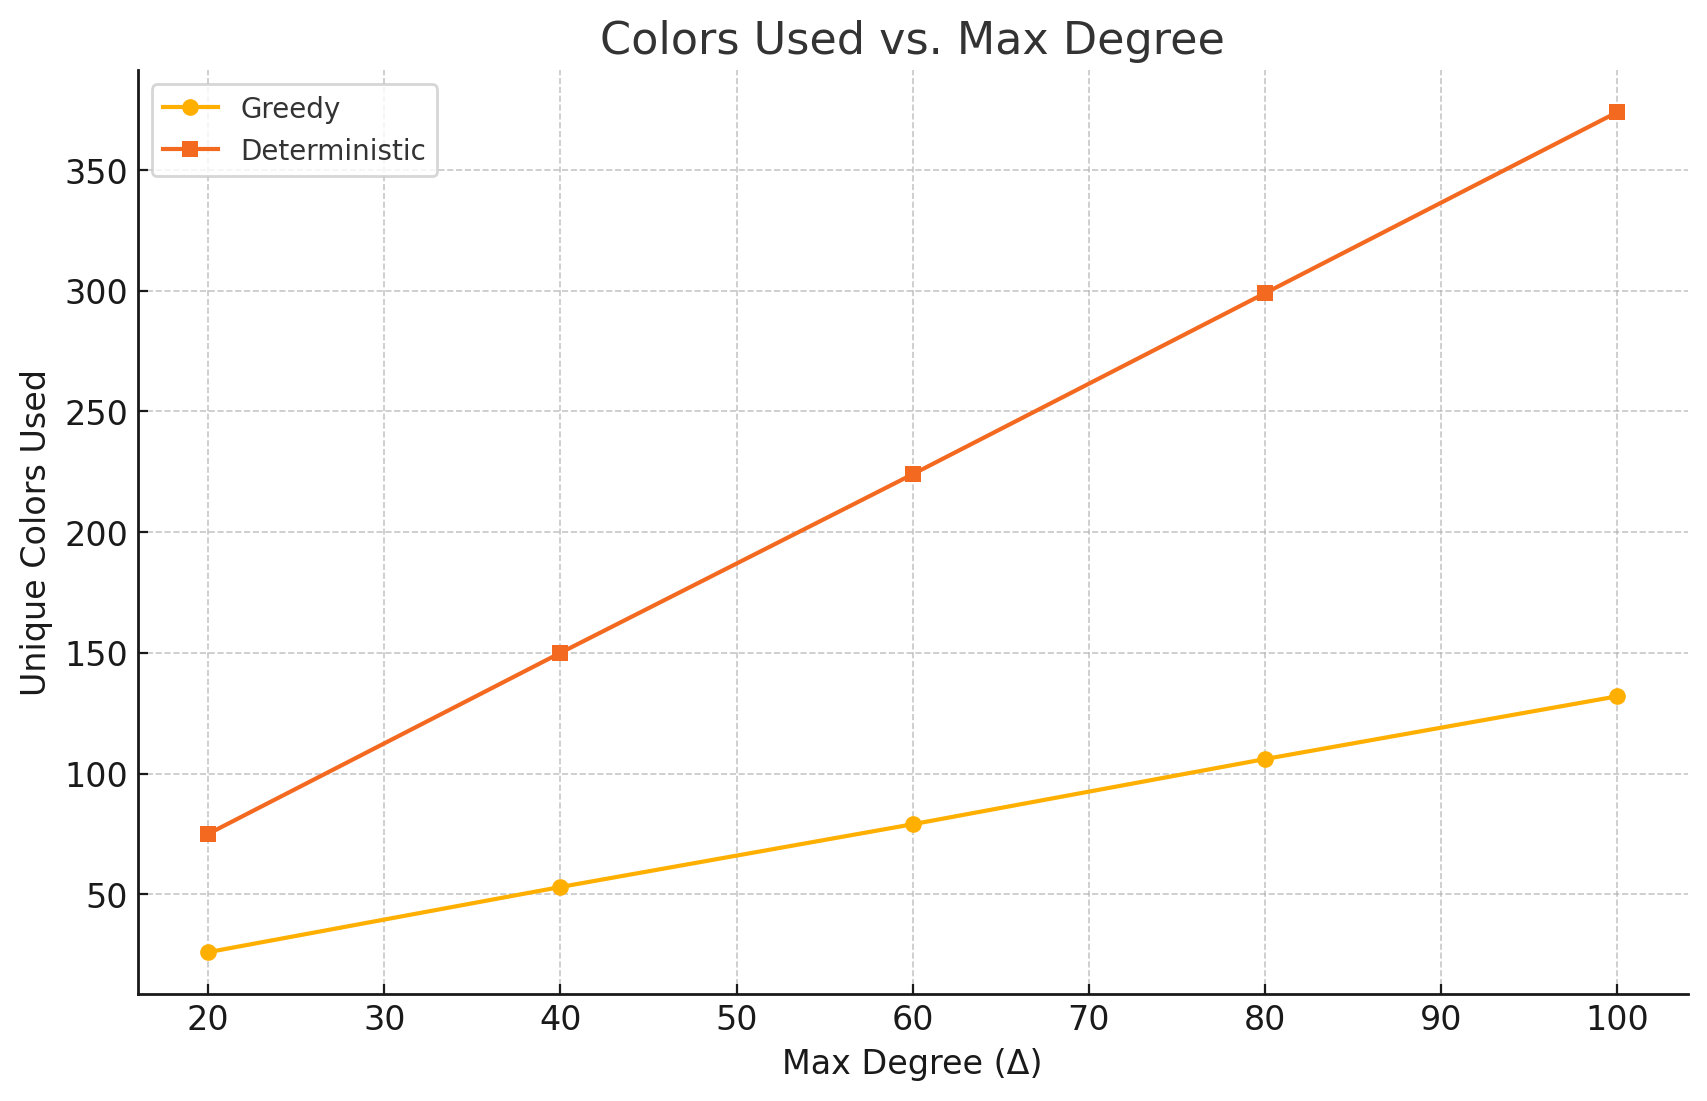
\includegraphics[width=0.5\linewidth]{color vs max dergee.png}
    \caption{Dense graphs}
    \label{fig:enter-label}
\end{figure}
  \item On sparse graphs or graphs with high degree variance, our algorithm matched greedy but rarely outperformed it.
\end{itemize}

\begin{figure}[H]
    \centering
    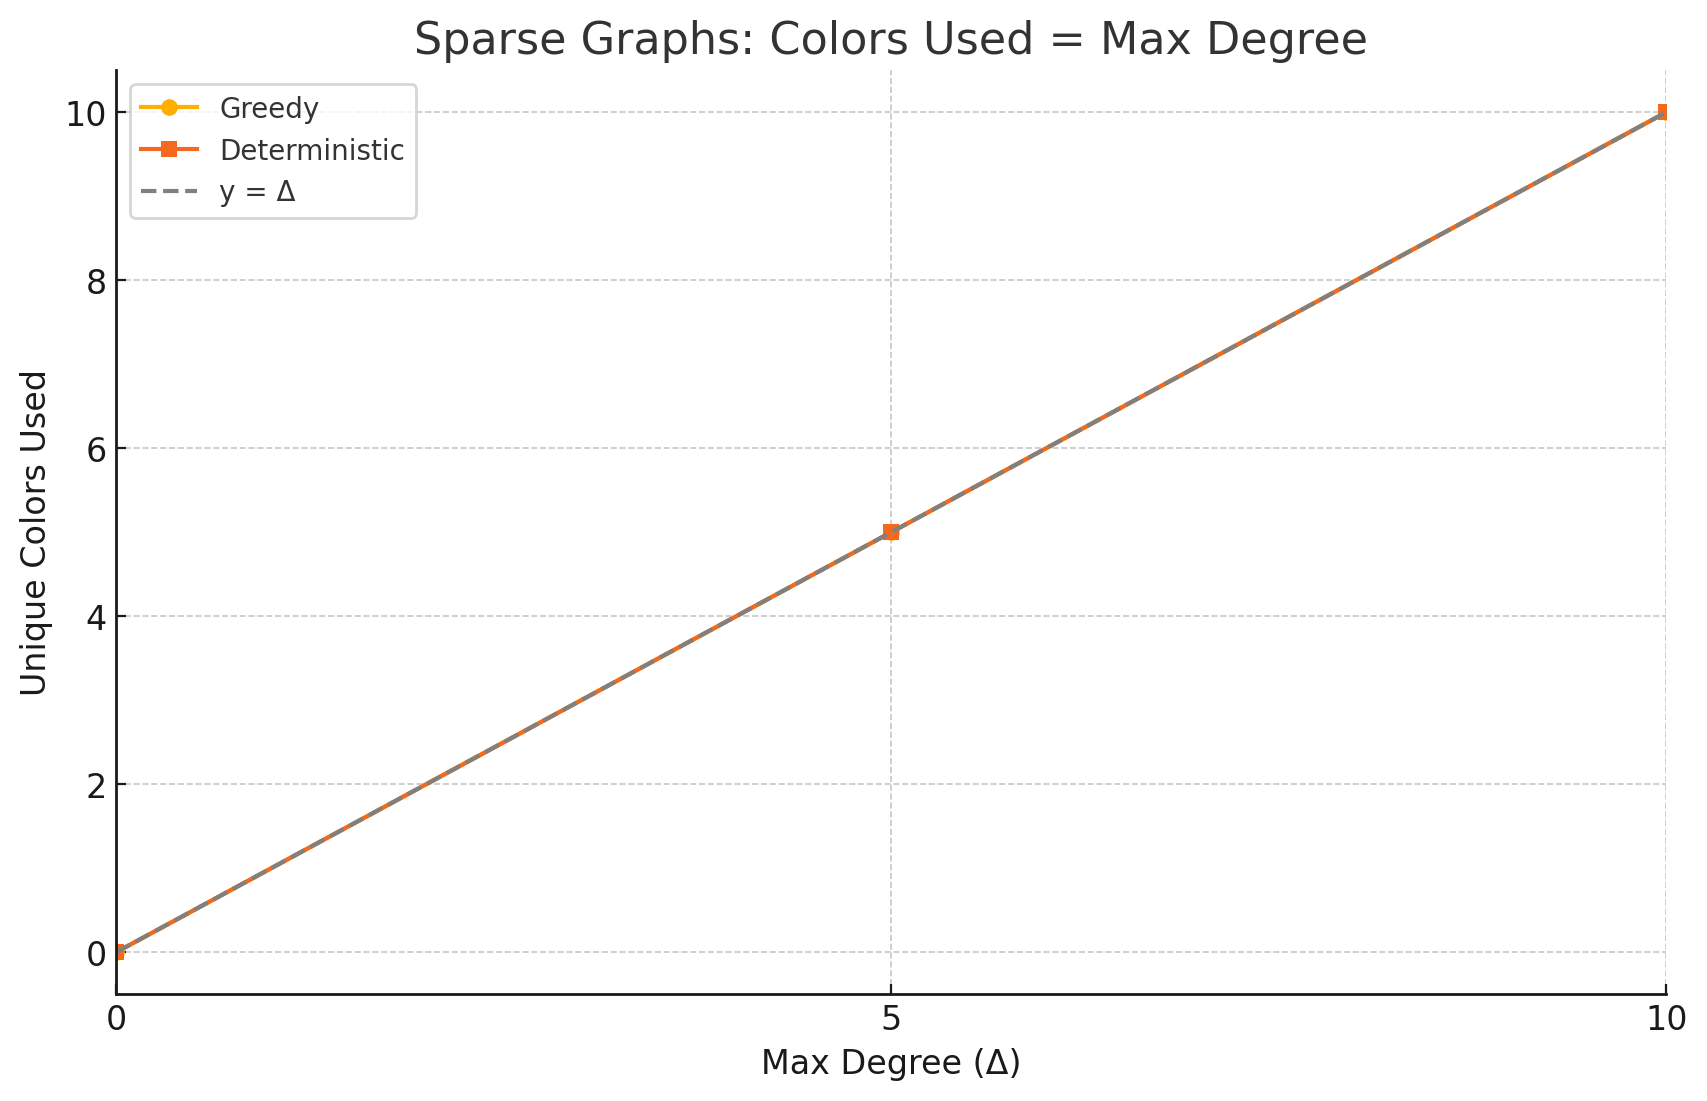
\includegraphics[width=0.5\linewidth]{sparse 1.png}
    \caption{Sparse Graph}
    \label{fig:enter-label}
\end{figure}

\section{Challenges \& Solutions}

\textbf{Key Challenges:}
\begin{itemize}
  \item Understanding the CRS mechanism in detail. Derandomization aspects such as pessimistic estimators and martingale bounds were difficult to fully implement.
  \item The paper lacked a reference implementation, making validation hard.
  \item We were unable to generate test cases where the theoretical advantage consistently manifested.
\end{itemize}

\textbf{Solutions Attempted:}
\begin{itemize}
  \item Implemented full partial coloring and greedy fallback.
  \item Read related literature to understand CRS more deeply.
  \item Tuned hyperparameters (e.g., palette size, offset thresholds).
\end{itemize}

\section{Enhancements}

  We have implemented and evaluated several practical enhancements to our baseline algorithm:

\begin{itemize}
  \item \textbf{Heuristic Palette‐Size.} 
    Replaced the theoretically‐derived
    \[
      \varepsilon = \tfrac{2}{5}\sqrt{\tfrac{\ln n}{\Delta}},
      \quad
      \text{palette\_size} = \bigl\lceil(1+\sqrt{\varepsilon})\Delta\bigr\rceil
    \]
    with the simpler, data‐driven rule
    \[
      \text{palette\_size} = \Delta + 4\,\log_{2}\!\Delta.
    \]
  
  
  \item \textbf{Raised Greedy‐Fallback Threshold.}
    Changed the recursion‐termination condition to apply more CRS rounds on denser subgraphs before reverting to the greedy fallback.
  
  \item \textbf{Fixed Palette Offset Strategy.}
    After each round, we increment the color‐block offset by
    \[
      \texttt{palette\_offset} \;+=\; 3\,\Delta,
    \]
    mirroring the paper’s “fresh color blocks” idea. 
\end{itemize}

\section{Further Plan}
\begin{itemize}
  \item \textbf{Restore the Theoretical Palette‐Size.}
    Replace our heuristic \(\Delta + 4\log_2\!\Delta\) rule with
    \(\lceil(1+\sqrt{\varepsilon})\Delta\rceil\) where
    \(\varepsilon=\tfrac25\sqrt{\tfrac{\ln n}{\Delta}}\), and verify
    its impact on color‐usage overhead.

  \item \textbf{Dynamic \(\varepsilon\) Scheduling.}
    Implement per‐round recomputation of \(\varepsilon_i\) as
    \(\tfrac25\sqrt{\tfrac{\ln n}{\Delta_i}}\), so that each CRS pass
    adapts to the current maximum degree \(\Delta_i\). 
\end{itemize}

\section{Conclusion}

While we have implemented the full structure of the deterministic algorithm proposed in the paper, our version does not achieve the expected competitive advantage over the greedy baseline. This is likely due to:
\begin{itemize}
  \item Gaps in understanding the exact derandomization process (e.g., simulating CRS with martingale guarantees).
  \item Absence of detailed construction for subroutines such as pessimistic estimators.
  \item No available reference code for comparison or correctness confirmation.
\end{itemize}

Despite these limitations, the implementation process provided deep insights into the complexity of competitive online algorithms and the challenges of derandomization in a practical setting.

\end{document}
